\documentclass[nopagenumber,9pt]{beamer}

\mode<presentation> {
  \usetheme[]{CambridgeUS}
  %\useoutertheme{shadow}
  \setbeamercovered{transparent}
  \usecolortheme{seahorse}
%\usecolortheme{sidebartab}
%  \usefonttheme{structurebold}
  \useinnertheme{default}
\useinnertheme{rounded}
}
\usepackage{nicefrac}
\RequirePackage{amsmath,amsfonts,amsthm}

\usepackage{float}
\usepackage[english]{babel}
\usepackage{amsmath}
\usepackage[utf8]{inputenc}
\usepackage{times}
\usepackage{url}
\usepackage[T1]{fontenc}
%\usepackage{multirow}
\usepackage{color}
\newcommand{\mb}[1]{\mathbf{#1}}
\usepackage{graphicx}
\graphicspath{{./figure/}}

\usepackage[ruled,vlined]{algorithm2e}
\usepackage{xcolor,colortbl}
\usepackage{rotating}
\usepackage{multirow}

\usepackage{tikz}
\usepackage{ulem}


\newtheorem{proposition}{Proposition}
\newcommand{\I}{\mathbb{I}}
\newcommand{\E}{\mathbb{E}}
\renewcommand{\P}{\mathbb{P}}
\newcommand{\R}{\mathbb{R}}
\newcommand{\bs}{\boldsymbol}
\newcommand{\bbeta}{\boldsymbol{\beta}}
\newcommand{\balpha}{\boldsymbol{\alpha}}
\newcommand{\btheta}{\boldsymbol{\theta}}
\newcommand{\bY}{\mathbf{Y}}
\newcommand{\bX}{\mathbf{X}}
\newcommand{\bZ}{\mathbf{Z}}
\newcommand{\by}{\mathbf{y}}
\newcommand{\bz}{\mathbf{z}}
\newcommand{\ba}{\mathbf{a}}
\newcommand{\bx}{\mathbf{x}}
\newcommand{\bh}{\mathbf{h}}
\newcommand{\bb}{\mathbf{b}}
\newcommand{\bB}{\mathbf{B}}
\newcommand{\bM}{\mathbf{M}}
\newcommand{\bphi}{\boldsymbol{\phi}}
\newcommand{\bpsi}{\boldsymbol{\psi}}
\newcommand{\bpi}{\boldsymbol{\pi}}
\newcommand{\btau}{\boldsymbol{\tau}}
\newcommand{\Ecal}{\mathcal{E}}
\newcommand{\GP}{\mathcal{GP}}
\newcommand{\bxi}{\boldsymbol{\xi}}
\newcommand{\brho}{\boldsymbol{\rho}}
\newcommand{\bgamma}{\boldsymbol{\gamma}}
\newcommand{\bsigma}{\boldsymbol{\sigma}}



\title[Introduction]{Calibration of computer models}

%titre premiere page

\subtitle{Introduction}

\author[P. Barbillon]{ Pierre \textsc{Barbillon}}
\bigskip

\date{Fall 2023}

\subject{Séminaire}



\AtBeginSection[] {
 \begin{frame}<beamer>
   \frametitle{Outline}
   \tableofcontents[currentsection]
  \end{frame}
}

\AtBeginSubsection[] {
\begin{frame}<beamer>
   \frametitle{Outline}
   \tableofcontents[currentsection,currentsubsection]
 \end{frame}
}


\begin{document}

\begin{frame}
\titlepage
%\includegraphics[scale=.12]{AgroParisTech_-_logo.PNG}
%\vspace{-1.5cm}
%\begin{flushright}
% \includegraphics[scale=.1]{Logotype-INRA-transparent.png}
% \end{flushright}
\vspace{-1cm}
\centering
\begin{tabular}{ccc}
 
\includegraphics[scale=.08]{LogoUPSaclay.jpg}&
  
\includegraphics[scale=1.3]{agrologo.png}&
   
\includegraphics[scale=.1]{LogoINRAE.jpg}
\end{tabular}


\end{frame}



\begin{frame}
\frametitle{Uncertainty Quantification / Model Uncertainty}

{\centering
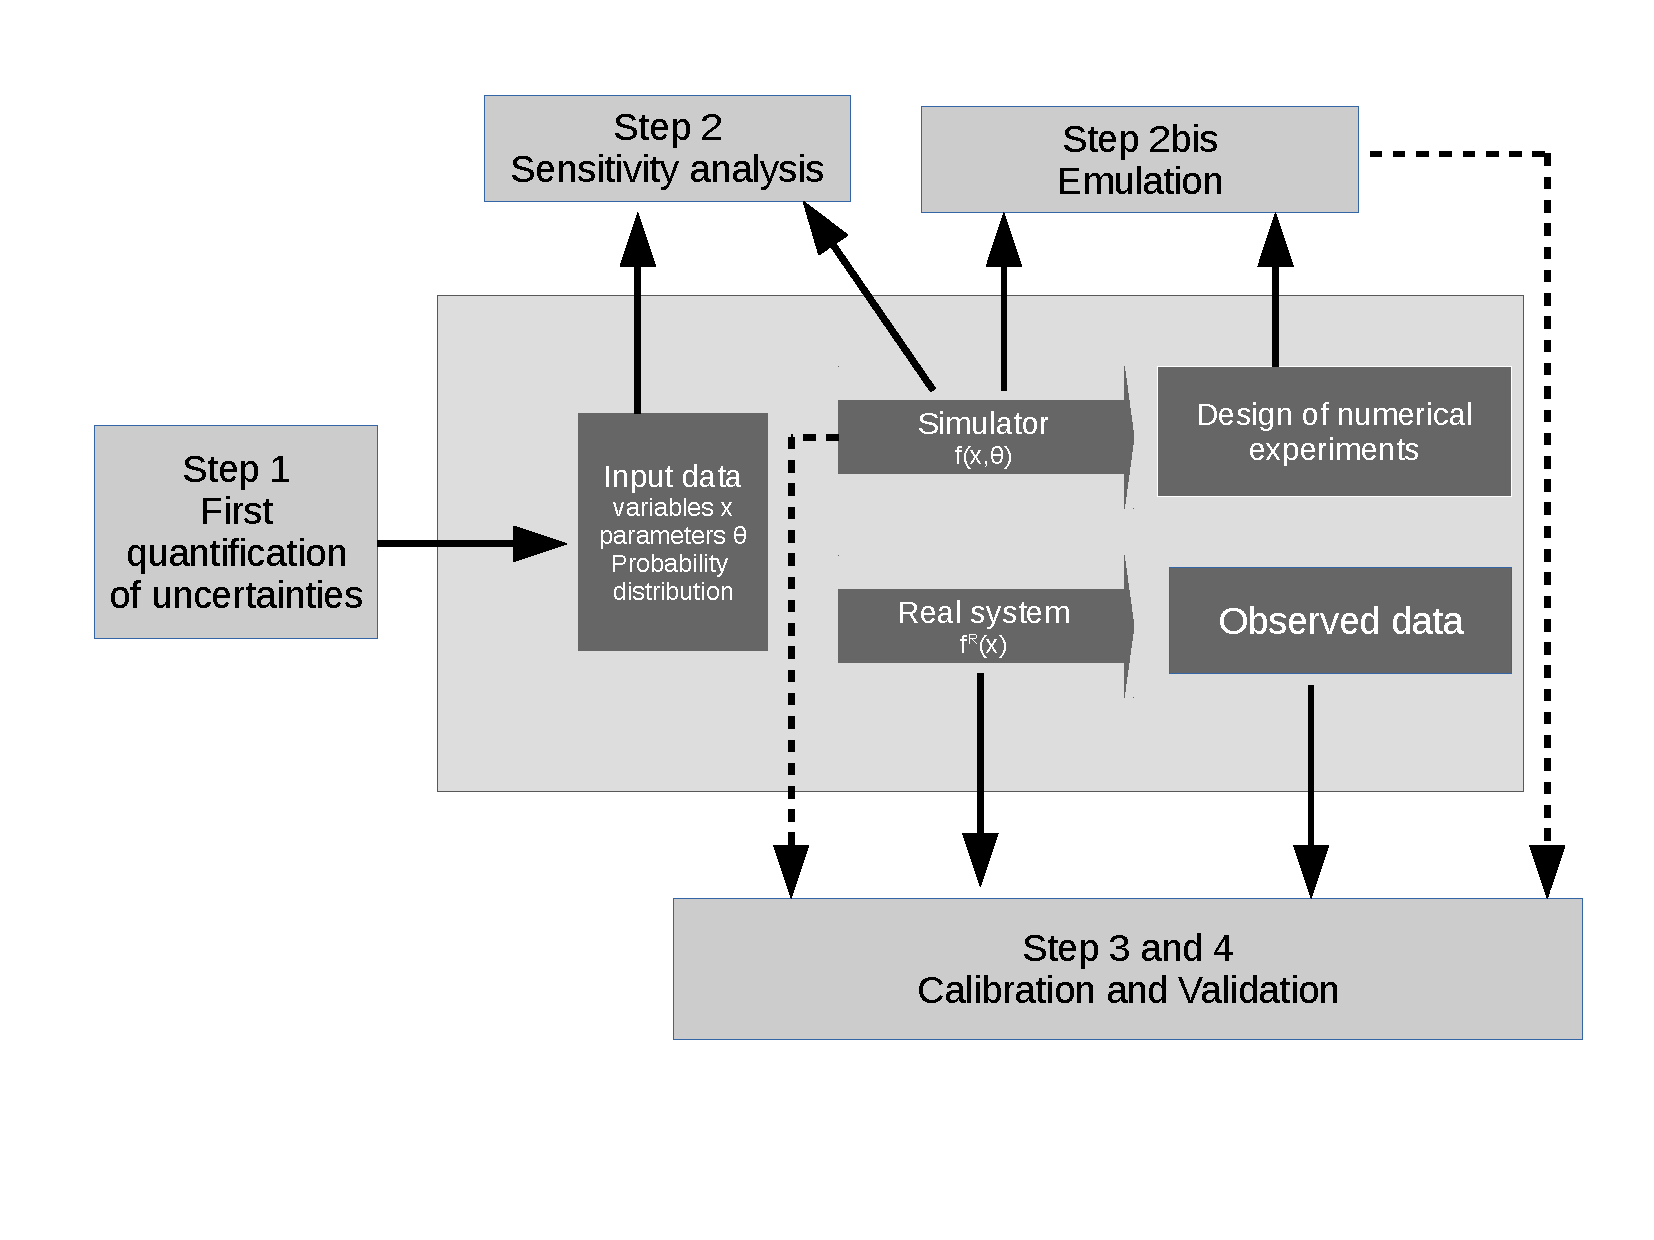
\includegraphics[scale=.25]{SchemaUQ.pdf}}


In this talk we will focus on calibration and validation.

\bigskip

Ref.: \color{blue} Kennedy and O'Hagan (2001), Hidgon et al. (2005), Bayarri et al. (2007)\color{black}.


\end{frame}



\begin{frame}
\frametitle{Calibration of a computer code} 
 \textbf{Computer experiments:}
 \\
 \medskip
Computer model (simulator)  $(\bx,\btheta)\mapsto f(\bx,\btheta)\in \mathbb{R}^s $ where\\
\medskip
\begin{itemize}
  \item \textbf{physical parameters}: $\bx\in  \mathbb{X}\subset\mathbb{R}^p$ observable and often controllable inputs
  \medskip
  \item \textbf{simulator parameters}: $\btheta\in \Theta\subset\mathbb{R}^d$ non-observable parameters, required to run the simulator.
  \\
  \smallskip
  2 types:
  \begin{itemize}
   \item ``calibration parameters'': physical meaning but unknown, necessary to make the code mimic the reality,  
   \item ``tuning parameters'': no physical interpretation.
  \end{itemize}
\end{itemize}

  \bigskip
  
  \textbf{Goal:}\\
  Calibrate the code: finding ``best'' or ``true'' $\btheta$ from real observations / field data 
  (provided by physical experiments):
  $$\by=\{y_1=\zeta(\bx_1),\ldots,y_n=\zeta(\bx_n)\}\,,$$  

  where $\zeta$ is the real physical phenomenon.
%   \textbf{Observations / Data:}
%   For different inputs: $\bx_1,\ldots,\bx_n$\\
  
  \end{frame}

  
  \begin{frame}
 \frametitle{Validation}
 \begin{itemize}
  \item Validation (rather than verification) is considered,
  \item[]
  \item Does the computer simulator correspond to field data?
  
  $$\exists \btheta^*?, \ \textrm{s.t.},\ \forall \bx,\quad f(\bx,\btheta^*)\approx y(\bx)$$
  
  \item[]
  
  
  \item This question is related with intended use of the simulator: range of $\bx$, required precision... 
  
  \item[]
  
%   \item The validation of the computer simulator depends on the known or unknown precision of the field data
%   
%   \item[]
  
  \item Biased computer model, no setting of calibrated parameters leads to outputs close to field data\\
  $\Rightarrow$ {\color{red} discrepancy}.\\
%   What is the meaning of validation
%   in that context?  
%   
  
  \item[]
  
 \item Do we want to validate the computer model itself or the computer model with the bias / discrepancy correction?
 \end{itemize}

\end{frame}

\end{document}
